%----------------------------------------------------------------------------
\chapter{Background}\label{ch:background}
%----------------------------------------------------------------------------

In this chapter I present the foundations of this work. In \autoref{sec:mbse}, I introduce the concept of model-based systems engineering, which is a well known approach for complex system design. This section also goes into detail about SysML (\autoref{ssec:sysml}), which is a widely used \emph{systems modeling language}. Next, I talk about the concept of formal verification in \autoref{sec:formal_verification}, and introduce Petri nets (\autoref{ssec:petri-net}) and a mapping between activities and Petri nets (\autoref{ssec:activities-as-petri-nets}). Lastly, I introduce the Gamma Statechart Composition Framework, which is a tool for modeling and verifying composite systems using statechart behaviours (\autoref{sec:gamma}), and a low-level formalism called XSTS (\autoref{sec:xsts}), used as an intermediary language for model checking by Gamma.

%----------------------------------------------------------------------------
\section{Model-based Systems Engineering}\label{sec:mbse}
%----------------------------------------------------------------------------

The INCOSE SE Vision 2020 defines Model-based systems engineering (MBSE) as:

\blockquote{the formalized application of modeling to support system requirements, design, analysis, verification and validation activities beginning in the conceptual design phase and continuing throughout development and later life cycle phases. MBSE is part of a long-term trend toward model-centric approaches adopted by other engineering disciplines, including mechanical, electrical and software. In particular, MBSE is expected to replace the document-centric approach that has been practiced by systems engineers in the past and to influence the future practice of systems engineering by being fully integrated into the definition of systems engineering processes. \cite{incose-systems-engineering-2020}}

Applying MBSE is expected to provide significant benefits over the document centric approach by enhancing productivity and quality, reducing risk, and providing improved communications among the system development team \cite{omgwiki}.

In MBSE, one of the most important concepts is the term \enquote{model} itself. Literature gives various definitions for models:

\begin{enumerate}
	\item A physical, mathematical, or otherwise logical representation of a system, entity, phenomenon, or process.\cite{DoD_modeling_and_simulation}\label{item:dod}
	\item A representation of one or more concepts that may be realized in the physical world \cite{sysml_practical_guide}.
	\item A simplified representation of a system at some particular point in time or space intended to promote understanding of the real system \cite{modsim}.
	\item An abstraction of a system, aimed at understanding, communicating, explaining, or designing aspects of interest of that system \cite{object-process-methodology}.
	\item A selective representation of some system whose form and content are chosen based on a specific set of concerns. The model is related to the system by an explicit or implicit mapping \cite{ORMSC/2010-09-06}.
\end{enumerate}

As one can see, choosing a definition is very much dependent upon how we wish to use our \enquote{model}; in this work I will use the \ref{item:dod}st definition.

\subsection{Systems Modeling Language}\label{ssec:sysml}

Systems Modeling Language (OMG SysML \cite{omg_sysml}) is a general-purpose modeling language that supports the specification, design, analysis, and verification of systems that may include harware and equipment, software, data, personnel, procedures, and facilities. SysML is a graphical modeling language with a semantic foundation for representing requirements, behaviour, structure, and properties of the system and its components \cite{sysml_practical_guide}.

This work focuses only on the \emph{behavioural} modeling tools SysML provides. In the following section, I present two of the most used concepts; State Machines and Activity Diagrams.

\subsubsection*{State Machine}

Reactive systems are all around us in our daily lives; in smart phones, avionics systems or event our calculators. Frequently, reactive systems appear in areas, where safety-critical operation is crucial, as even the slightest
misbehaviour can have catastrophic consequences. This makes the verification of these systems a must during their design process.

The defining characteristic of reactive systems is their event-driven nature, which means that they continuously receive external stimuli (\emph{events}), based on which they change their internal \emph{state} and possibly react with some output \cite{10.1007/978-3-642-82453-1_17}. Reactive systems can be verified using model checking techniques (see \autoref{sec:formal_verification}). Statecharts \cite{HAREL1987231} are a popular and intuitive language to capture the behaviour of reactive systems \cite{10.1145/3417990.3421407, 10.1007/978-3-319-11653-2_10}, while also being formally defined.

\begin{figure}[!ht]
	\centering
	\includesvg[inkscapelatex=false, width=130mm, keepaspectratio]{traffic-light-ctrl-sm}
	\caption{SysML State Machine describing the behaviour of a traffic light controller.}
	\label{fig:sysml_state_machine}
\end{figure}

SysML state machines extend the concept of statecharts with hierarchical state-refinement, orthogonal regions, action-effect behaviour and state machine composition. These advanced abstraction constructs make state machines easy to use for engineers, but hinder their formal verification. This abstraction gap can be bridged using a transformation tool, such as Gamma, of which I will be talking in \autoref{sec:gamma}.

\autoref{fig:sysml_state_machine} shows a state machine modeling the behaviour of a traffic light controller. The \emph{TrafficLightCtrl} component has three ports, two inputs (\emph{Control} and \emph{PoliceInterrupt}) for user input, and one output (\emph{LightCommands}) for controlling the specific light it is connected to. The state machine changes between the \emph{red}-\emph{green}\emph{yellow} lights, upon a \emph{toggle} command. However, if a \emph{police} signal is received, it starts turning on and off the yellow light every 500ms.

\subsubsection*{Activity Diagram}\label{ssec:sysml_activity}

State machines cannot describe the complicated semantics of distributed systems with concurrent, parallel behaviour, where the \emph{interesting} thing is what the system \emph{does} step-by-step. SysML activity diagrams are a primary representation for modeling process based behaviour \cite{omg_sysml} for distributed, concurrent systems. \autoref{fig:sysml_activity_artifacts} shows the set of interesting modeling elements used in this work. In the following, I introduce the different artifacts of SysML activities and show an example of a SysML activity diagram.

\begin{figure}[!ht]
	\centering
	\includesvg[inkscapelatex=false, width=110mm, keepaspectratio]{sysml-activity-artifacts}
	\caption{Artifacts of SysML activity diagrams.}
	\label{fig:sysml_activity_artifacts}
\end{figure}

SysML activity diagram is a graph based model, where the nodes are connected via flows. The dynamic behaviour of activity diagrams comes from \emph{tokens} travelling from node to node; based on the given node's semantics, a connected flow removes tokens from the source node and puts them onto the target node. Flows can also have \emph{guards}, which are expressions specifying when the given flow is \emph{enabled} or not; only enabled nodes can transfer tokens.

Tokens are a way of creating limitations over which node can run, and which cannot; a given node is considered \emph{running}, only when it contains a token. Tokens \emph{flow} between nodes, carrying with them a given value - this value can be of type \emph{void}, which makes it a \emph{control} token.

The different nodes represent the different semantic \enquote{tools} at our disposal; they can represent different actions, or introduce interesting token flow semantics.
Simple \textbf{actions} represent a single step of behaviour that convert a set of inputs to a set of outputs. Both inputs and outputs are specified as pins, which get their data from connected flows - making that flow a \emph{data flow}. The flow starts from the initial node, and ends with a \emph{Flow Final} or \emph{Activity Final} node. \emph{Fork} nodes generate tokens on all of their output flows, and \emph{Join} nodes forward the tokens, only when all input flows contain one - thus, the two nodes come in a \emph{pair}. On the other hand, \emph{Merge} nodes do not wait for all flows, they forward any token they receive instantly. Likewise, \emph{Decision} nodes take one token from its input flows, and sends it out on its single enabled output flow.

The detailed specification for SysML Activity Diagrams can be found in the OMG specification \cite{omg_sysml}.

\begin{figure}[!ht]
	\centering
	\includesvg[inkscapelatex=false, width=130mm, keepaspectratio]{activity-running-example}
	\caption{The activity of editing, compiling and linking two files.}
	\label{fig:activity-running-example}
\end{figure}

\autoref{fig:activity-running-example} shows an example activity diagram, modeling the process of editing, compiling and linking two files. First, the files have to be read, after which they are \emph{transfered} to the compiler module. We want to compile the two different files in \emph{parallel}, thus we split the control flow using a \emph{fork} node. Once the files are compiled, we link both of them - since linking requires both files, it is preceded by a \emph{join} node. Finally, if the resulting code contains errors, we \emph{edit} the source files and start over - otherwise we are done.

\iffalse
\subsubsection{Differences and Combination}

State Machines are a popular [1, 2] language to capture the behaviour
of reactive systems\cite{HAREL1987231} that react to external stimuli depending on
their internal state. Stat Machines provide an expressive formalism to
represent complex \emph{state-based} behaviour by introducing hierarchical
state refinement, memory (variables and history state) and complex
transitions (e.g., fork and join transitions).

As contrast, Activities model the behaviour of distributed systems with many interconnecting components, all running in parallel; said components may have dependencies on each other (one calculates a value the other needs), or have a limited resources (a factory only has one worker).

SysML provides a functionality to combine different behaviours, using the \emph{call behaviour} pattern. By using a call behaviour action inside a State Machine, we are able to combine the behaviour of the two. This is the basis of composite behaviour models, and the motivation of this work. 
\fi
%%----------------------------------------------------------------------------
\section{Verifcation Techniques in Systems Engineering}\label{sec:mbse-verification}
%----------------------------------------------------------------------------

Using Model-based Systems Engineering helps reduce the amount of time needed to develop complicated systems, however, as all development processes, it is still prone to human error. In the section I introduce a typical engineering workflow based on the widely known V-model. This workflow is used as a general guideline in the development of safety-critical systems, however, many variants have been developed for the special needs of the different sectors. The V-model defines the elementary steps and draws a general workflow for the design and implementation of the system as depicted on Figure 1.2. In addition, the workflow defines verification and validation steps in the development to the correctness of the system. 

As you can see in \autoref{fig:v-model}, the workflow is split into multiple phases, all of which having their own \emph{design}, \emph{implementation} and \emph{verification} steps. The first phase is requirement design, where the requirements of the system are identified and collected. In the second phase, designing the architecture provides the necessary decomposition to be able to construct the component level design. At each phase, the designer refines the result of the former phases by providing more details. As the result of the final phase in the left wing, the implementation is produced for each design. The implementation has to be tested and verified against coding and other implementation errors. After the component level validation, system integration builds the smaller pieces together where extensive integration testing is executed to validate that the components work properly together. Finally, system validation ensures that the system is indeed what the customer desires.
%----------------------------------------------------------------------------
\section{Formal Verification}\label{sec:formal_verification}
%----------------------------------------------------------------------------

In order to raise the reliability of system analysis, a system analysis technique is required that can have the precision of paper-and-pencil based mathematical proofs, and thus does not rely upon computer-arithmetic, and utilizes the computers for bookkeeping, to be able to handle complex systems without having to worry about human-errors. Formal verification methods, which are primarily based on theoretical computer science fundamentals like logic calculi, automata theory and strongly type systems, fulfil these requirements. The main principle behind formal analysis of a system is to construct a computer based mathematical model of the given system and formally verify, within a computer, that this model meets rigorous specifications of intended behaviour. Due to the mathematical nature of the analysis, 100\% accuracy can be guaranteed.\cite{https://doi:10.4018/978-1-4666-5888-2.ch705}

\subsection{Model Checking}

\emph{Model Checking} is a formal verification method to verify properties of finite systems, i.e., to decide whether a given formal model \(M\) satisfies a given requirement \(\gamma\) or not. The name comes from formal logic, where a logical formula may have zero or more models, which define the interpretation of the symbols used in the formula and the base set such that the formula is true. In this sense, the question is whether the formal model is indeed a model of the formal requirement: \(M \models \gamma\)?

Model Checker algorithms (see \autoref{fig:model_checking}), such as UPPAAL\footnote{https://uppaal.org/}\cite{uppaal} or Theta\footnote{https://inf.mit.bme.hu/en/theta}\cite{theta} use SAT solvers to answer this question; and can even return a \emph{proof} (i.e., a part of the model) that \(M\) indeed does satisfy said requirement\footnote{These proofs usually come in the form of an execution trace}.

\begin{figure}[!ht]
	\centering
	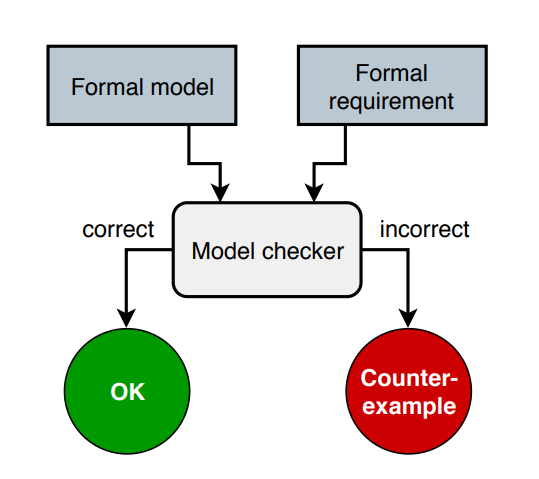
\includegraphics[width=67mm, keepaspectratio]{figures/model_checking.png}\hspace{1cm}
	\caption{An illustration of model checking.}
	\label{fig:model_checking}
\end{figure}

\subsection{Petri Net}

\begin{figure}[!ht]
	\centering
	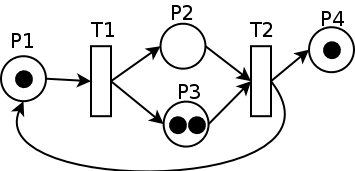
\includegraphics[width=67mm, keepaspectratio]{figures/petri_net.png}\hspace{1cm}
	\caption{An example Petri net with 2 transitions and 4 places.}
	\label{fig:petri_net}
\end{figure}

Petri nets are a widely used formalism to model concurrent, asynchronous systems \cite{24143}. The formal definition of a Petri net (including inhibitor arcs) is as follows (see \autoref{fig:petri_net} for an illustration of the notations).

\begin{definition}[Petri net]
	
	A Petri net is a tuple \( PN = (P, T, W, M_0) \)
	
	\begin{itemize}
		\item \(P\) is the set of \emph{places} (defining state variables);
		\item \(T\) is the set of \emph{transitions} (defining behaviour), such that \( P \bigcap T = \emptyset \);
		\item \(W \subseteq W^+ \bigcup W^- \) is a set of two types of arcs, where \(  W^+ : T \times P \rightarrow \mathbb{N}\) and \( W^- : P \times T \rightarrow \mathbb{N} \) are the set of input arcs and output arcs, respectively (\( \mathbb{N} \) is the set of all natural numbers);
		\item \(M_0 : P \rightarrow \mathbb{N} \) is the \emph{initial marking}, i.e., the number of \emph{tokens} on each place.
	\end{itemize}
\end{definition}

The state of a Petri net is defined by the current marking \( M : P \rightarrow \mathbb{N} \). The behaviour of the systems is described as follows. A transition \( t \) is enabled if \( \forall p \in P : M(p) \in W(p, t) \). Any enabled transition \(t\) may fire non-deterministically, creating the new marking \( M' \) of the Petri as follows: \( \forall p \in P : M'(p) = M(p) - W^-(p, t) + W^+(t, p) \).

In words: W describes the \emph{weight} of each flow from a transition to a place, or from a place to a transition. Firing a transition \(t\) in a marking \(M\) consumes \(W^-(p_i, t)\) tokens from each of its input places \(p_i\), and produces \(W(t, p_o)\) tokens in each of its output places \(p_o\). One such transition \(t\) is \emph{enabled} (it may \emph{fire}) in \(M\) if there are enough tokens in its input places for the consumptions to be possible, i.e., if and only if \( \forall p : M(p) \ge W(s, t)\).

\subsection{Activities as Petri Nets}

As I have mentioned in the beginning of this Section, formal verification requires models to be specified using \emph{mathematical} precision. In the paper called "Verifying SysML activity diagrams using formal transformation to Petri nets"\cite{https://doi.org/10.1002/sys.21524} by Edward Huang, Leon F. McGinnis and Steven W. Mitchell they propose a way to \emph{partially} map SysML activity diagrams to Petri nets. In the following, I will summarise their work.

\subsubsection*{Constrained Sub-set of SysML}

Since SysML Activity Diagrams do not have exact execution semantics\cite{euml}, the PN mapping can only be done for a limited subset of the modeling elements: actions, initial nodes, final nodes, join nodes, fork nodes, merge nodes, decision nodes, pins and object/control flows, which have precise execution semantics as defined in the Foundational Subset for Executable UML Models.\cite{fuml}

The other constraints are:

\begin{enumerate}
	\item The value of tokens is not considered.
	\item Control flows with multiple tokens at a time are not considered.
	\item Optional object/control flows are not considered, i.e., multiplicity lower bounds are strictly positive.
\end{enumerate}

As a result of these constraints, the exact semantics of activities cannot be described using only Petri nets. This fact will be addressed in \autoref{ch:activiy_verification}.

\subsubsection*{Mapping Rules}

The paper groups the given elements into two sets: "load-and-send" (LAS) and "immediate-repeat" (IR)

LAS nodes are fired when all their inputs have tokens equal to or more than the weight function (in PN) or the multiplicity lower bounds (in activity diagrams). When an LAS node fires,the number of tokens (equal to the weight function or the multiplicity lower bound) associated with an input arcs/pin is consumed and the number of tokens (equal to the weight function or the multiplicity lower bound) associated with an output arc/pin is added. Examples of LAS nodes in PN are transitions.

In contrast, as soon as an IR node receives a token from any input, it immediately adds a token to its output nodes. Places in PN are an example of IR nodes.

%----------------------------------------------------------------------------
\section{The Gamma Statechart Composition Framework}\label{sec:gamma}
%----------------------------------------------------------------------------

The Gamma Statechart Composition Framework\footnote{https://inf.mit.bme.hu/en/gamma} \cite{mixed_statecharts_2020} is an integrated tool to support the design, verification and validation as well as code generation for component-based reactive systems. The behaviour of each component is captured by a statechart, while assembling the system from components is driven by a domain-specific composition language\footnote{The composition language be the \emph{ibd} model in SysML}. Gamma supports formal verification by mapping composite statecharts to a back-end model checker. Execution traces obtained as witnesses during verification are back-annotated as test cases to replay an error trace or to validate external code generators~\cite{molnar2018gamma}. 

\begin{figure}[!ht]
	\centering
	\includesvg[inkscapelatex=false, width=120mm, keepaspectratio]{gamma-functionality-overview}
	\caption{The overview of model transformation chains and modeling languages of the Gamma framework \cite{mixed_statecharts_2020}. The parts relevant to this work have been marked with red outline.}
	\label{fig:gamma-overview}
\end{figure}

The workflow of Gamma builds on a model transformation chain depicted in \autoref{fig:gamma-overview}, which illustrates the input and output models of these model transformations as well as the languages in which they are defined, and the relations between them. The modeling languages are as follows.

\begin{itemize}
	\item The \textbf{Gamma Statechart Language (GSL)} is a UML/SysML-based statechart language supporting different semantic variants of statecharts.
	\item The \textbf{Gamma Composition Language (GCL)} is a composition language for the formal hierarchical composition of state-based 	components according to multiple execution and interaction semantics.
	\item The \textbf{Gamma Genmodel Language (GGL)} is a configuration language for configuring model transformations.
	\item The \textbf{Gamma Property Language (GPL)} is a property language supporting the definition (CTL*) properties and thus, the formal specification of requirements regarding (composite)	component behavior.
	\item The \textbf{Gamma Trace Language (GTL)} is a high-level specification language for  execution traces of (composite) components.
\end{itemize}

Optionally, statechart models defined in supported modeling tools (front-ends) can be imported into Gamma (Step 1), which can be integrated according to well-defined execution and interaction semantics (Step 2). The resulting composite model is processed and transformed into the input formalisms of integrated model checker back-ends (Step 3). The model checker back-ends provide witnesses (diagnostic traces) based on specified properties, which are back-annotated, resulting in abstract traces (Step 4).
Finally, the abstract traces are mapped into concrete (executable) traces tailored to the targeted execution environment (Step 5). For a more detailed description, see \cite{mixed_statecharts_2020}.

\subsection{Example Statechart}

\autoref{lst:gamma-statechart} shows the Gamma Statechart representation of the State Machine introduced in \autoref{fig:sysml_state_machine}.

\begin{lstlisting}[float,language=statechart, caption={The traffic light controller state machine in the Gamma textual representation.}, label={lst:gamma-statechart}]
package TrafficLightCtrl
import "Interfaces"
statechart TrafficLightCtrl [
	port Control : requires Control
	port PoliceInterrupt : requires PoliceInterrupt
	port LightCommands : provides LightCommands
] {
	timeout BlinkingYellowTimeout3
	timeout BlackTimeout4
	transition from Yellow to Red when Control.toggle
	transition from Normal to Interrupted when PoliceInterrupt.police
	// ...
	transition from BlinkingYellow to Black when timeout BlinkingYellowTimeout3
	transition from Black to BlinkingYellow when timeout BlackTimeout4
	region main_region {
		state Normal {
			region normal {
				shallow history Entry2
				state Green {
					entry / raise LightCommands.displayGreen;
				}
				state Red {
					entry / raise LightCommands.displayRed;
				}
				state Yellow {
					entry / raise LightCommands.displayYellow;
				}
			}
		}
		state Interrupted {
			region interrupted {
				initial Entry1
				state Black {
					entry / set BlackTimeout4 := 500 ms; 
						raise LightCommands.displayNone;
				}
				state BlinkingYellow {
					entry / set BlinkingYellowTimeout3 := 500 ms; 
						raise LightCommands.displayYellow;
				}
			}
		}
		initial Entry0
	}
}
\end{lstlisting}
%----------------------------------------------------------------------------
\section{Extended Symbolic Transition System}\label{sec:xsts}
%----------------------------------------------------------------------------

The high-level nature of engineering models means they are easy-to-use for engineers, but leads to difficulties during the formal verification process. SysML state machines and acitivty diagrams for example contain high-level  constructs that make the modeling workflow more intuitive and enable the modeling of significantly more complex systems, however they are difficult to process using formal methods that are defined on low-level mathematical formalism and verified using SMT solvers. In this section, I introduce the XSTS\cite{xsts} language, which is a low-level modeling formalism designed to bridge the aforementioned gap between engineering models and formal methods.

\subsection{Formal definition}

\begin{definition}[Extended symbolic transition system]
	
	An \emph{Extended symbolic transition system} is a tuple \( XSTS = (D, V, V_C, IV, Tr, In, En) \), where:
	
	\begin{itemize}
		\item \(D = \{ D_{v1}, D_{v2}, \dots, D_{vn} \} \) is a set of value domains;
		\item \(V = \{ v_1, v_2, \dots, v_n \} \) is a set of variables with domains \(D_{v1}, D_{v2}, \dots, D_{vn}\);
		\item \(V_C \subseteq V\) is a set of variables marked as \emph{control variables};
		\item \(IV \in D_{v1} \times D_{v2} \times \dots \times D_{vn}\) is the \emph{initial value function} used to describe the initial state. The initial value function \(IV\) assigns an initial value \(IV(v) \in D_v\) to variables \(v \in V\) of their domain \(D_v\);
		\item \(Tr \subseteq Ops\) is a set of operations, representing the \emph{internal transition relation}; it describes the internal behaviour of the system;
		\item \(In \subseteq Ops\) is a set of operations, representing the \emph{initialisation transition relation}; it is used to describe more complex initialisation, and is executed once and only once, at the very beginning;
		\item \(En \subseteq Ops\) is a set of operations, representing the \emph{environmental transition relation}; it is used to model the system's interactions with its environment.
	\end{itemize}
\end{definition}\label{def:xsts}

In any state of the system a single operation is selected from the sets introduced above (\(Tr\), \(In\) and \(En\)). The set from where the operation can be selected depends on the current state: In the initial state - (which is described by the initialization vector \(IV\)) - only operations from the \(In\) set can be executed. Operations from the \(In\) set can only fire in the initial state and nowhere else. After that, \(En\) and \(Tr\) are selected in an alternating manner.

Operations \(op \in Ops\) describe the transitions between states of the system, where \(Ops\) is the set of all possible transitions. All operations are atomic in the sense that they are either executed in their entirety or none at all. XSTS defines the following operations:

\paragraph{Basic operations}

Basic operations contain no inner (nested) operations. \textbf{Assignments} assign a given value \(v\) from domain \(D_n\) to variable \(V_n\). \textbf{Havocs} behave likewise, except the value is not predetermined; giving a way to assign random value to a variable. Lastly, \textbf{assumptions} check a condition, and can only be executed if their condition evaluates to \emph{true}.

\paragraph{Composite operations}

Composite operations contain other operations, and can be used to describe complex control stuctures. Note that while these are composite operations, their execution is still atomic; meaning that an \emph{assume} operation prevents its containing operations from firing. \textbf{Sequences} are essentially multiple operations executed after each other, while \textbf{parallels} execute all operations at the same time. And lastly, \textbf{choices} model non-deterministic choices between multiple operations; one and only one branch of the choice operation is selected for execution, but that selected operation can still only be executed atomically - e.g., a single failing assume operation can prevent execution.

\subsection{Simple example}

Below is an example XSTS model defined in the language. For a more exact presentation please see \autoref{sec:xsts_language} in the Appendix.

\begin{Verbatim}
	itt majd egy szép xsts példa lesz a running example-re (vagy valami hasonlóra). 
	Akár lehetne egy Gamma által generált statechart is.
\end{Verbatim}


%----------------------------------------------------------------------------
\section{Kapcsolódó munkák}
%----------------------------------------------------------------------------

% TODO


